\documentclass[11pt]{article}
\renewcommand{\arraystretch}{1.5} % Default value: 1
\usepackage{sectsty}
\allsectionsfont{\color{blue}\fontfamily{lmss}\selectfont}
\usepackage{fontspec}
\setmainfont{XCharter}

\usepackage{listings}
\lstset{
basicstyle=\small\ttfamily,
tabsize=8,
columns=flexible,
breaklines=true,
frame=tb,
rulecolor=\color[rgb]{0.8,0.8,0.7},
backgroundcolor=\color[rgb]{1,1,0.91},
postbreak=\raisebox{0ex}[0ex][0ex]{\ensuremath{\color{red}\hookrightarrow\space}}
}
\usepackage{fontawesome}


\usepackage{mdframed}
\newmdenv[
  backgroundcolor=gray,
  fontcolor=white,
  nobreak=true,
]{terminalinput}



\usepackage{parskip}
\usepackage{float}



    \usepackage[T1]{fontenc}
    % Nicer default font than Computer Modern for most use cases
    \usepackage{palatino}

    % Basic figure setup, for now with no caption control since it's done
    % automatically by Pandoc (which extracts ![](path) syntax from Markdown).
    \usepackage{graphicx}
    % We will generate all images so they have a width \maxwidth. This means
    % that they will get their normal width if they fit onto the page, but
    % are scaled down if they would overflow the margins.
    \makeatletter
    \def\maxwidth{\ifdim\Gin@nat@width>\linewidth\linewidth
    \else\Gin@nat@width\fi}
    \makeatother
    \let\Oldincludegraphics\includegraphics
    % Set max figure width to be 80% of text width, for now hardcoded.
\renewcommand{\includegraphics}[1]{\Oldincludegraphics[width=.8\maxwidth, height=.55\textheight, keepaspectratio]{#1}}
    % Ensure that by default, figures have no caption (until we provide a
    % proper Figure object with a Caption API and a way to capture that
    % in the conversion process - todo).
    \usepackage{caption}
    \DeclareCaptionLabelFormat{nolabel}{}
    \captionsetup{labelformat=nolabel, textfont=bf}

    \usepackage{adjustbox} % Used to constrain images to a maximum size
    \usepackage{xcolor} % Allow colors to be defined
    \usepackage{enumerate} % Needed for markdown enumerations to work
    \usepackage{geometry} % Used to adjust the document margins
    \usepackage{amsmath} % Equations
    \usepackage{amssymb} % Equations
    \usepackage{textcomp} % defines textquotesingle
    % Hack from http://tex.stackexchange.com/a/47451/13684:
    \AtBeginDocument{%
        \def\PYZsq{\textquotesingle}% Upright quotes in Pygmentized code
    }
    \usepackage{upquote} % Upright quotes for verbatim code
    \usepackage{eurosym} % defines \euro
    \usepackage[mathletters]{ucs} % Extended unicode (utf-8) support
    \usepackage[utf8x]{inputenc} % Allow utf-8 characters in the tex document
    \usepackage{fancyvrb} % verbatim replacement that allows latex
    \usepackage{grffile} % extends the file name processing of package graphics
                         % to support a larger range
    % The hyperref package gives us a pdf with properly built
    % internal navigation ('pdf bookmarks' for the table of contents,
    % internal cross-reference links, web links for URLs, etc.)
    \usepackage{hyperref}
    \usepackage{longtable} % longtable support required by pandoc >1.10
    \usepackage{booktabs}  % table support for pandoc > 1.12.2
    \usepackage[normalem]{ulem} % ulem is needed to support strikethroughs (\sout)
                                % normalem makes italics be italics, not underlines




    % Colors for the hyperref package
    \definecolor{urlcolor}{rgb}{0,.145,.698}
    \definecolor{linkcolor}{rgb}{.71,0.21,0.01}
    \definecolor{citecolor}{rgb}{.12,.54,.11}

    % ANSI colors
    \definecolor{ansi-black}{HTML}{3E424D}
    \definecolor{ansi-black-intense}{HTML}{282C36}
    \definecolor{ansi-red}{HTML}{E75C58}
    \definecolor{ansi-red-intense}{HTML}{B22B31}
    \definecolor{ansi-green}{HTML}{00A250}
    \definecolor{ansi-green-intense}{HTML}{007427}
    \definecolor{ansi-yellow}{HTML}{DDB62B}
    \definecolor{ansi-yellow-intense}{HTML}{B27D12}
    \definecolor{ansi-blue}{HTML}{208FFB}
    \definecolor{ansi-blue-intense}{HTML}{0065CA}
    \definecolor{ansi-magenta}{HTML}{D160C4}
    \definecolor{ansi-magenta-intense}{HTML}{A03196}
    \definecolor{ansi-cyan}{HTML}{60C6C8}
    \definecolor{ansi-cyan-intense}{HTML}{258F8F}
    \definecolor{ansi-white}{HTML}{C5C1B4}
    \definecolor{ansi-white-intense}{HTML}{A1A6B2}

    % commands and environments needed by pandoc snippets
    % extracted from the output of `pandoc -s`
    \providecommand{\tightlist}{%
      \setlength{\itemsep}{0pt}\setlength{\parskip}{0pt}}
    \DefineVerbatimEnvironment{Highlighting}{Verbatim}{commandchars=\\\{\}}
    % Add ',fontsize=\small' for more characters per line
    \newenvironment{Shaded}{}{}
    \newcommand{\KeywordTok}[1]{\textcolor[rgb]{0.00,0.44,0.13}{\textbf{{#1}}}}
    \newcommand{\DataTypeTok}[1]{\textcolor[rgb]{0.56,0.13,0.00}{{#1}}}
    \newcommand{\DecValTok}[1]{\textcolor[rgb]{0.25,0.63,0.44}{{#1}}}
    \newcommand{\BaseNTok}[1]{\textcolor[rgb]{0.25,0.63,0.44}{{#1}}}
    \newcommand{\FloatTok}[1]{\textcolor[rgb]{0.25,0.63,0.44}{{#1}}}
    \newcommand{\CharTok}[1]{\textcolor[rgb]{0.25,0.44,0.63}{{#1}}}
    \newcommand{\StringTok}[1]{\textcolor[rgb]{0.25,0.44,0.63}{{#1}}}
    \newcommand{\CommentTok}[1]{\textcolor[rgb]{0.38,0.63,0.69}{\textit{{#1}}}}
    \newcommand{\OtherTok}[1]{\textcolor[rgb]{0.00,0.44,0.13}{{#1}}}
    \newcommand{\AlertTok}[1]{\textcolor[rgb]{1.00,0.00,0.00}{\textbf{{#1}}}}
    \newcommand{\FunctionTok}[1]{\textcolor[rgb]{0.02,0.16,0.49}{{#1}}}
    \newcommand{\RegionMarkerTok}[1]{{#1}}
    \newcommand{\ErrorTok}[1]{\textcolor[rgb]{1.00,0.00,0.00}{\textbf{{#1}}}}
    \newcommand{\NormalTok}[1]{{#1}}

    % Additional commands for more recent versions of Pandoc
    \newcommand{\ConstantTok}[1]{\textcolor[rgb]{0.53,0.00,0.00}{{#1}}}
    \newcommand{\SpecialCharTok}[1]{\textcolor[rgb]{0.25,0.44,0.63}{{#1}}}
    \newcommand{\VerbatimStringTok}[1]{\textcolor[rgb]{0.25,0.44,0.63}{{#1}}}
    \newcommand{\SpecialStringTok}[1]{\textcolor[rgb]{0.73,0.40,0.53}{{#1}}}
    \newcommand{\ImportTok}[1]{{#1}}
    \newcommand{\DocumentationTok}[1]{\textcolor[rgb]{0.73,0.13,0.13}{\textit{{#1}}}}
    \newcommand{\AnnotationTok}[1]{\textcolor[rgb]{0.38,0.63,0.69}{\textbf{\textit{{#1}}}}}
    \newcommand{\CommentVarTok}[1]{\textcolor[rgb]{0.38,0.63,0.69}{\textbf{\textit{{#1}}}}}
    \newcommand{\VariableTok}[1]{\textcolor[rgb]{0.10,0.09,0.49}{{#1}}}
    \newcommand{\ControlFlowTok}[1]{\textcolor[rgb]{0.00,0.44,0.13}{\textbf{{#1}}}}
    \newcommand{\OperatorTok}[1]{\textcolor[rgb]{0.40,0.40,0.40}{{#1}}}
    \newcommand{\BuiltInTok}[1]{{#1}}
    \newcommand{\ExtensionTok}[1]{{#1}}
    \newcommand{\PreprocessorTok}[1]{\textcolor[rgb]{0.74,0.48,0.00}{{#1}}}
    \newcommand{\AttributeTok}[1]{\textcolor[rgb]{0.49,0.56,0.16}{{#1}}}
    \newcommand{\InformationTok}[1]{\textcolor[rgb]{0.38,0.63,0.69}{\textbf{\textit{{#1}}}}}
    \newcommand{\WarningTok}[1]{\textcolor[rgb]{0.38,0.63,0.69}{\textbf{\textit{{#1}}}}}


    % Define a nice break command that doesn't care if a line doesn't already
    % exist.
    \def\br{\hspace*{\fill} \\* }
    % Math Jax compatability definitions
    \def\gt{>}
    \def\lt{<}
    % Document parameters
    \title{index}




    % Pygments definitions

\makeatletter
\def\PY@reset{\let\PY@it=\relax \let\PY@bf=\relax%
    \let\PY@ul=\relax \let\PY@tc=\relax%
    \let\PY@bc=\relax \let\PY@ff=\relax}
\def\PY@tok#1{\csname PY@tok@#1\endcsname}
\def\PY@toks#1+{\ifx\relax#1\empty\else%
    \PY@tok{#1}\expandafter\PY@toks\fi}
\def\PY@do#1{\PY@bc{\PY@tc{\PY@ul{%
    \PY@it{\PY@bf{\PY@ff{#1}}}}}}}
\def\PY#1#2{\PY@reset\PY@toks#1+\relax+\PY@do{#2}}

\expandafter\def\csname PY@tok@w\endcsname{\def\PY@tc##1{\textcolor[rgb]{0.73,0.73,0.73}{##1}}}
\expandafter\def\csname PY@tok@c\endcsname{\let\PY@it=\textit\def\PY@tc##1{\textcolor[rgb]{0.25,0.50,0.50}{##1}}}
\expandafter\def\csname PY@tok@cp\endcsname{\def\PY@tc##1{\textcolor[rgb]{0.74,0.48,0.00}{##1}}}
\expandafter\def\csname PY@tok@k\endcsname{\let\PY@bf=\textbf\def\PY@tc##1{\textcolor[rgb]{0.00,0.50,0.00}{##1}}}
\expandafter\def\csname PY@tok@kp\endcsname{\def\PY@tc##1{\textcolor[rgb]{0.00,0.50,0.00}{##1}}}
\expandafter\def\csname PY@tok@kt\endcsname{\def\PY@tc##1{\textcolor[rgb]{0.69,0.00,0.25}{##1}}}
\expandafter\def\csname PY@tok@o\endcsname{\def\PY@tc##1{\textcolor[rgb]{0.40,0.40,0.40}{##1}}}
\expandafter\def\csname PY@tok@ow\endcsname{\let\PY@bf=\textbf\def\PY@tc##1{\textcolor[rgb]{0.67,0.13,1.00}{##1}}}
\expandafter\def\csname PY@tok@nb\endcsname{\def\PY@tc##1{\textcolor[rgb]{0.00,0.50,0.00}{##1}}}
\expandafter\def\csname PY@tok@nf\endcsname{\def\PY@tc##1{\textcolor[rgb]{0.00,0.00,1.00}{##1}}}
\expandafter\def\csname PY@tok@nc\endcsname{\let\PY@bf=\textbf\def\PY@tc##1{\textcolor[rgb]{0.00,0.00,1.00}{##1}}}
\expandafter\def\csname PY@tok@nn\endcsname{\let\PY@bf=\textbf\def\PY@tc##1{\textcolor[rgb]{0.00,0.00,1.00}{##1}}}
\expandafter\def\csname PY@tok@ne\endcsname{\let\PY@bf=\textbf\def\PY@tc##1{\textcolor[rgb]{0.82,0.25,0.23}{##1}}}
\expandafter\def\csname PY@tok@nv\endcsname{\def\PY@tc##1{\textcolor[rgb]{0.10,0.09,0.49}{##1}}}
\expandafter\def\csname PY@tok@no\endcsname{\def\PY@tc##1{\textcolor[rgb]{0.53,0.00,0.00}{##1}}}
\expandafter\def\csname PY@tok@nl\endcsname{\def\PY@tc##1{\textcolor[rgb]{0.63,0.63,0.00}{##1}}}
\expandafter\def\csname PY@tok@ni\endcsname{\let\PY@bf=\textbf\def\PY@tc##1{\textcolor[rgb]{0.60,0.60,0.60}{##1}}}
\expandafter\def\csname PY@tok@na\endcsname{\def\PY@tc##1{\textcolor[rgb]{0.49,0.56,0.16}{##1}}}
\expandafter\def\csname PY@tok@nt\endcsname{\let\PY@bf=\textbf\def\PY@tc##1{\textcolor[rgb]{0.00,0.50,0.00}{##1}}}
\expandafter\def\csname PY@tok@nd\endcsname{\def\PY@tc##1{\textcolor[rgb]{0.67,0.13,1.00}{##1}}}
\expandafter\def\csname PY@tok@s\endcsname{\def\PY@tc##1{\textcolor[rgb]{0.73,0.13,0.13}{##1}}}
\expandafter\def\csname PY@tok@sd\endcsname{\let\PY@it=\textit\def\PY@tc##1{\textcolor[rgb]{0.73,0.13,0.13}{##1}}}
\expandafter\def\csname PY@tok@si\endcsname{\let\PY@bf=\textbf\def\PY@tc##1{\textcolor[rgb]{0.73,0.40,0.53}{##1}}}
\expandafter\def\csname PY@tok@se\endcsname{\let\PY@bf=\textbf\def\PY@tc##1{\textcolor[rgb]{0.73,0.40,0.13}{##1}}}
\expandafter\def\csname PY@tok@sr\endcsname{\def\PY@tc##1{\textcolor[rgb]{0.73,0.40,0.53}{##1}}}
\expandafter\def\csname PY@tok@ss\endcsname{\def\PY@tc##1{\textcolor[rgb]{0.10,0.09,0.49}{##1}}}
\expandafter\def\csname PY@tok@sx\endcsname{\def\PY@tc##1{\textcolor[rgb]{0.00,0.50,0.00}{##1}}}
\expandafter\def\csname PY@tok@m\endcsname{\def\PY@tc##1{\textcolor[rgb]{0.40,0.40,0.40}{##1}}}
\expandafter\def\csname PY@tok@gh\endcsname{\let\PY@bf=\textbf\def\PY@tc##1{\textcolor[rgb]{0.00,0.00,0.50}{##1}}}
\expandafter\def\csname PY@tok@gu\endcsname{\let\PY@bf=\textbf\def\PY@tc##1{\textcolor[rgb]{0.50,0.00,0.50}{##1}}}
\expandafter\def\csname PY@tok@gd\endcsname{\def\PY@tc##1{\textcolor[rgb]{0.63,0.00,0.00}{##1}}}
\expandafter\def\csname PY@tok@gi\endcsname{\def\PY@tc##1{\textcolor[rgb]{0.00,0.63,0.00}{##1}}}
\expandafter\def\csname PY@tok@gr\endcsname{\def\PY@tc##1{\textcolor[rgb]{1.00,0.00,0.00}{##1}}}
\expandafter\def\csname PY@tok@ge\endcsname{\let\PY@it=\textit}
\expandafter\def\csname PY@tok@gs\endcsname{\let\PY@bf=\textbf}
\expandafter\def\csname PY@tok@gp\endcsname{\let\PY@bf=\textbf\def\PY@tc##1{\textcolor[rgb]{0.00,0.00,0.50}{##1}}}
\expandafter\def\csname PY@tok@go\endcsname{\def\PY@tc##1{\textcolor[rgb]{0.53,0.53,0.53}{##1}}}
\expandafter\def\csname PY@tok@gt\endcsname{\def\PY@tc##1{\textcolor[rgb]{0.00,0.27,0.87}{##1}}}
\expandafter\def\csname PY@tok@err\endcsname{\def\PY@bc##1{\setlength{\fboxsep}{0pt}\fcolorbox[rgb]{1.00,0.00,0.00}{1,1,1}{\strut ##1}}}
\expandafter\def\csname PY@tok@kc\endcsname{\let\PY@bf=\textbf\def\PY@tc##1{\textcolor[rgb]{0.00,0.50,0.00}{##1}}}
\expandafter\def\csname PY@tok@kd\endcsname{\let\PY@bf=\textbf\def\PY@tc##1{\textcolor[rgb]{0.00,0.50,0.00}{##1}}}
\expandafter\def\csname PY@tok@kn\endcsname{\let\PY@bf=\textbf\def\PY@tc##1{\textcolor[rgb]{0.00,0.50,0.00}{##1}}}
\expandafter\def\csname PY@tok@kr\endcsname{\let\PY@bf=\textbf\def\PY@tc##1{\textcolor[rgb]{0.00,0.50,0.00}{##1}}}
\expandafter\def\csname PY@tok@bp\endcsname{\def\PY@tc##1{\textcolor[rgb]{0.00,0.50,0.00}{##1}}}
\expandafter\def\csname PY@tok@vc\endcsname{\def\PY@tc##1{\textcolor[rgb]{0.10,0.09,0.49}{##1}}}
\expandafter\def\csname PY@tok@vg\endcsname{\def\PY@tc##1{\textcolor[rgb]{0.10,0.09,0.49}{##1}}}
\expandafter\def\csname PY@tok@vi\endcsname{\def\PY@tc##1{\textcolor[rgb]{0.10,0.09,0.49}{##1}}}
\expandafter\def\csname PY@tok@sb\endcsname{\def\PY@tc##1{\textcolor[rgb]{0.73,0.13,0.13}{##1}}}
\expandafter\def\csname PY@tok@sc\endcsname{\def\PY@tc##1{\textcolor[rgb]{0.73,0.13,0.13}{##1}}}
\expandafter\def\csname PY@tok@s2\endcsname{\def\PY@tc##1{\textcolor[rgb]{0.73,0.13,0.13}{##1}}}
\expandafter\def\csname PY@tok@sh\endcsname{\def\PY@tc##1{\textcolor[rgb]{0.73,0.13,0.13}{##1}}}
\expandafter\def\csname PY@tok@s1\endcsname{\def\PY@tc##1{\textcolor[rgb]{0.73,0.13,0.13}{##1}}}
\expandafter\def\csname PY@tok@mb\endcsname{\def\PY@tc##1{\textcolor[rgb]{0.40,0.40,0.40}{##1}}}
\expandafter\def\csname PY@tok@mf\endcsname{\def\PY@tc##1{\textcolor[rgb]{0.40,0.40,0.40}{##1}}}
\expandafter\def\csname PY@tok@mh\endcsname{\def\PY@tc##1{\textcolor[rgb]{0.40,0.40,0.40}{##1}}}
\expandafter\def\csname PY@tok@mi\endcsname{\def\PY@tc##1{\textcolor[rgb]{0.40,0.40,0.40}{##1}}}
\expandafter\def\csname PY@tok@il\endcsname{\def\PY@tc##1{\textcolor[rgb]{0.40,0.40,0.40}{##1}}}
\expandafter\def\csname PY@tok@mo\endcsname{\def\PY@tc##1{\textcolor[rgb]{0.40,0.40,0.40}{##1}}}
\expandafter\def\csname PY@tok@ch\endcsname{\let\PY@it=\textit\def\PY@tc##1{\textcolor[rgb]{0.25,0.50,0.50}{##1}}}
\expandafter\def\csname PY@tok@cm\endcsname{\let\PY@it=\textit\def\PY@tc##1{\textcolor[rgb]{0.25,0.50,0.50}{##1}}}
\expandafter\def\csname PY@tok@cpf\endcsname{\let\PY@it=\textit\def\PY@tc##1{\textcolor[rgb]{0.25,0.50,0.50}{##1}}}
\expandafter\def\csname PY@tok@c1\endcsname{\let\PY@it=\textit\def\PY@tc##1{\textcolor[rgb]{0.25,0.50,0.50}{##1}}}
\expandafter\def\csname PY@tok@cs\endcsname{\let\PY@it=\textit\def\PY@tc##1{\textcolor[rgb]{0.25,0.50,0.50}{##1}}}

\def\PYZbs{\char`\\}
\def\PYZus{\char`\_}
\def\PYZob{\char`\{}
\def\PYZcb{\char`\}}
\def\PYZca{\char`\^}
\def\PYZam{\char`\&}
\def\PYZlt{\char`\<}
\def\PYZgt{\char`\>}
\def\PYZsh{\char`\#}
\def\PYZpc{\char`\%}
\def\PYZdl{\char`\$}
\def\PYZhy{\char`\-}
\def\PYZsq{\char`\'}
\def\PYZdq{\char`\"}
\def\PYZti{\char`\~}
% for compatibility with earlier versions
\def\PYZat{@}
\def\PYZlb{[}
\def\PYZrb{]}
\makeatother


    % Exact colors from NB
    \definecolor{incolor}{rgb}{0.0, 0.0, 0.5}
    \definecolor{outcolor}{rgb}{0.545, 0.0, 0.0}




    % Prevent overflowing lines due to hard-to-break entities
    \sloppy
    % Setup hyperref package
    \hypersetup{
      breaklinks=true,  % so long urls are correctly broken across lines
      colorlinks=true,
      urlcolor=urlcolor,
      linkcolor=linkcolor,
      citecolor=citecolor,
      }
    % Slightly bigger margins than the latex defaults

    \geometry{verbose,tmargin=1in,bmargin=1in,lmargin=1in,rmargin=1in}



\renewcommand{\PY}[2]{{#2}}
\usepackage{fancyhdr}
\pagestyle{fancy}
\rhead{\color{gray}\sf\small\rightmark}
\lhead{\nouppercase{\color{gray}\sf\small\leftmark}}
\cfoot{\color{gray}\sf\thepage}
\renewcommand{\footrulewidth}{1pt}
\begin{document}






    \hypertarget{pangenome-construction-using-roary}{%
\section{Pangenome Construction using
Roary}\label{pangenome-construction-using-roary}}

\hypertarget{introduction}{%
\subsection{Introduction}\label{introduction}}

Given a set of genomes, the pan genome is the collection of all genes
the set contains. Roary, the pan genome pipeline, takes closely related
annotated genomes in GFF3 file format and calculates the pan genome.

For more in depht information about Roary, please feel free to have a
look the paper:

\begin{quote}
\textbf{Roary: Rapid large-scale prokaryote pan genome analysis}\\
Andrew J. Page, Carla A. Cummins, Martin Hunt, Vanessa K. Wong, Sandra
Reuter, Matthew T. G. Holden, Maria Fookes, Daniel Falush, Jacqueline A.
Keane, Julian Parkhill\\
\textit{Bioinformatics, 2015;31(22):3691-3693
doi:\href{http://bioinformatics.oxfordjournals.org/content/31/22/3691}{10.1093/bioinformatics/btv421}}
\end{quote}

or visit the \href{http://sanger-pathogens.github.io/Roary/}{Roary
manual}.

\hypertarget{learning-outcomes}{%
\subsection{Learning outcomes}\label{learning-outcomes}}

By the end of this tutorial you can expect to be able to:

\begin{itemize}
\tightlist
\item
  Describe what a pangenome is
\item
  Prepare data for input to Roary
\item
  Perform QC on input data and understand why QC is important
\item
  Run Roary to create a pangenome with and without a core alignment
\item
  Understand the different output files produced by Roary
\item
  Draw a basic tree from the core gene alignment produced by Roary
\item
  Query the pangenome results produced by Roary
\item
  Use Phandango to visualise the results produced by Roary
\end{itemize}

\hypertarget{tutorial-sections}{%
\subsection{Tutorial sections}\label{tutorial-sections}}

This tutorial comprises the following sections:\\
1. \href{pan_genome.ipynb}{What is a pan genome}\\
2. \href{prepare_data.ipynb}{Preparing the input data}\\
3. \href{qc.ipynb}{Performing QC on your data}\\
4. \href{run_roary.ipynb}{Running Roary}\\
5. \href{results.ipynb}{Exploring the results}\\
6. \href{phandango.ipynb}{Visualising the results with Phandango}

\hypertarget{authors}{%
\subsection{Authors}\label{authors}}

This tutorial was created by \href{https://github.com/ssjunnebo}{Sara
Sjunnebo}.

\hypertarget{running-the-commands-from-this-tutorial}{%
\subsection{Running the commands from this
tutorial}\label{running-the-commands-from-this-tutorial}}

You can run the commands in this tutorial either directly from the
Jupyter notebook (if using Jupyter), or by typing the commands in your
terminal window.

\hypertarget{running-commands-on-jupyter}{%
\subsubsection{Running commands on
Jupyter}\label{running-commands-on-jupyter}}

If you are using Jupyter, command cells (like the one below) can be run
by selecting the cell and clicking \textit{Cell -\textgreater{} Run} from
the menu above or using \textit{ctrl Enter} to run the command. Let's give
this a try by printing our working directory using the \textit{pwd}
command and listing the files within it. Run the commands in the two
cells below.

\begin{terminalinput}
\begin{Verbatim}[commandchars=\\\{\}]
\llap{\color{black}\LARGE\faKeyboardO\hspace{1em}} \PY{n+nb}{pwd}
\end{Verbatim}
\end{terminalinput}

\begin{terminalinput}
\begin{Verbatim}[commandchars=\\\{\}]
\llap{\color{black}\LARGE\faKeyboardO\hspace{1em}} ls \PYZhy{}l
\end{Verbatim}
\end{terminalinput}

    \hypertarget{running-commands-in-the-terminal}{%
\subsubsection{Running commands in the
terminal}\label{running-commands-in-the-terminal}}

You can also follow this tutorial by typing all the commands you see
into a terminal window. This is similar to the ``Command Prompt'' window
on MS Windows systems, which allows the user to type DOS commands to
manage files.

To get started, select the cell below with the mouse and then either
press control and enter or choose Cell -\textgreater{} Run in the menu
at the top of the page.

\begin{terminalinput}
\begin{Verbatim}[commandchars=\\\{\}]
\llap{\color{black}\LARGE\faKeyboardO\hspace{1em}} \PY{n+nb}{echo} \PY{n+nb}{cd} \PY{n+nv}{\PYZdl{}PWD}
\end{Verbatim}
\end{terminalinput}

    Now open a new terminal on your computer and type the command that was
output by the previous cell followed by the enter key. The command will
look similar to this:

\begin{verbatim}
cd /home/manager/pathogen-informatics-training/Notebooks/ROARY/
\end{verbatim}

Now you can follow the instructions in the tutorial from here.

\hypertarget{lets-get-started}{%
\subsection{Let's get started!}\label{lets-get-started}}

This tutorial assumes that you have Roary and Prokka installed on your
computer. For download and installation instructions, please see:

\begin{itemize}
\tightlist
\item
  The \href{https://github.com/sanger-pathogens/roary}{Roary
  GitHub-page}
\item
  The \href{https://github.com/tseemann/prokka}{Prokka GitHub-page}
\end{itemize}

To check that you have installed Roary correctly, you can run the
following command:

\begin{terminalinput}
\begin{Verbatim}[commandchars=\\\{\}]
\llap{\color{black}\LARGE\faKeyboardO\hspace{1em}} roary \PYZhy{}\PYZhy{}help
\end{Verbatim}
\end{terminalinput}

    This should return the help message for Roary.

Similarly, to check that you have installed Prokka correctly, you can
run:

\begin{terminalinput}
\begin{Verbatim}[commandchars=\\\{\}]
\llap{\color{black}\LARGE\faKeyboardO\hspace{1em}} prokka \PYZhy{}\PYZhy{}help
\end{Verbatim}
\end{terminalinput}

    This should return the help message for Prokka.

    To get started with the tutorial, head to the first section:
\href{pan_genome.ipynb}{What is a pan genome}\\
The answers to all questions in the tutorial can be found
\href{answers.ipynb}{here}.


    % Add a bibliography block to the postdoc



\newpage






    \hypertarget{the-pan-genome}{%
\section{The Pan Genome}\label{the-pan-genome}}

The pan genome for a prokaryote population is the complete set of genes
that it contains. This includes genes present in all of the genomes, and
genes that are only present in some, or even only in one of the genomes.
The subset of genes present in all of the genomes is called the
\textbf{core genome}. These are often highly conserved genes with
important functions, for instance housekeeping genes. The subset of
genes that are not present in all, but in two or more of the genomes, is
called the \textbf{accessory genome}. The accessory genome often
contains genes that have been transferred between baterial strains, for
example genes linked to virulence or drug resistance. Genes present in
only one of the genomes can be referred to as \textbf{strain specific}.

    \begin{figure}[!h]
\centering
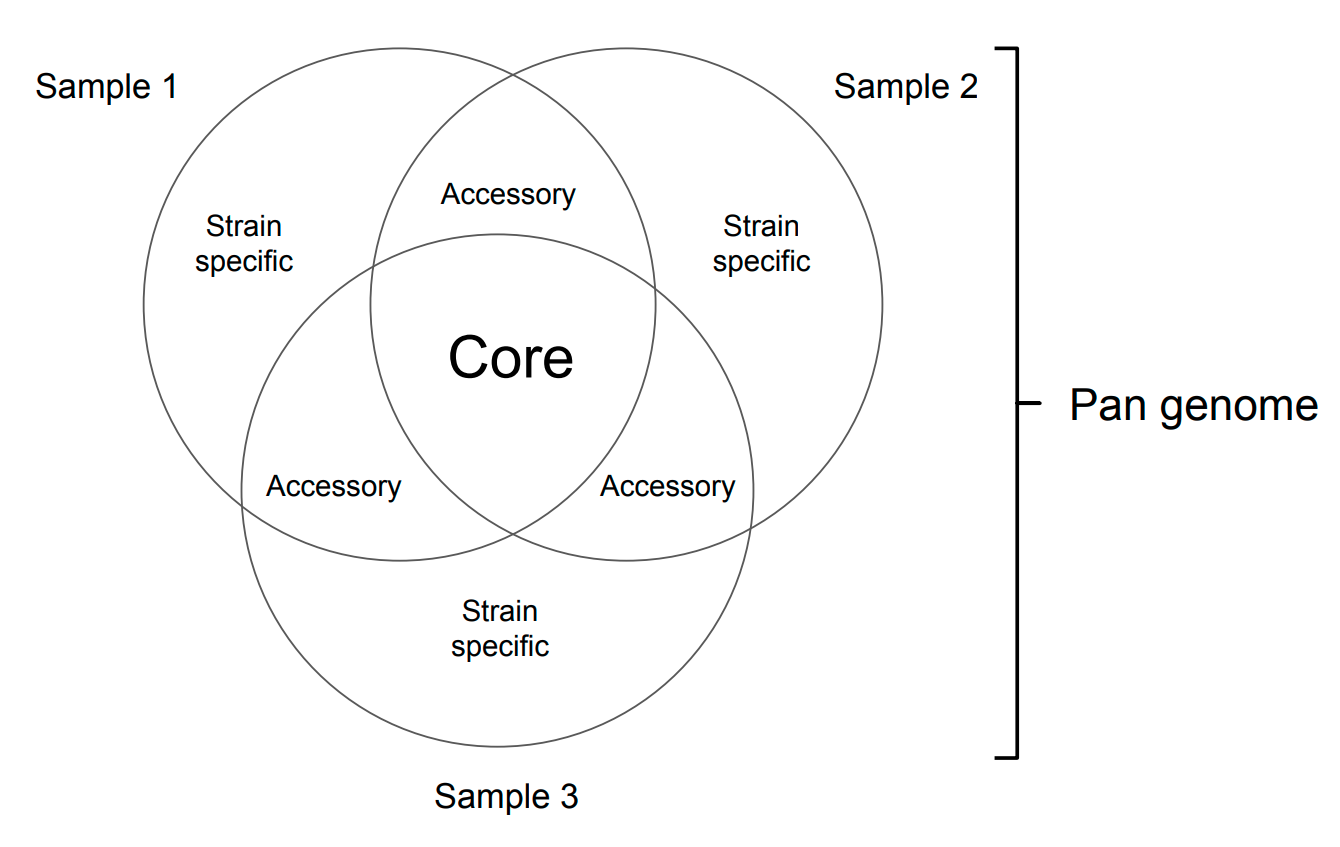
\includegraphics{img/pangenome.png}
\caption{Pan genome}
\end{figure}

    As you can imagine, the pan, core and acessory genomes can provide
important insight into the genetic structure of prokaryotic genomes. By
analysing the pan genome we can gain a better understanding of key
processes like evolution and selection. Roay is a software tool that
allows you to calculate the pan genome from annotated bacterial genomes.
It is fast and accurate and can conveniently be run on most modern PCs.
In this tutorial we are going to guide you through a complete pan genome
analysis, starting with annotation of the genomes, working through
running the pan genome pipelin, and finally visualising the results.

\hypertarget{check-your-understanding}{%
\subsection{Check your understanding}\label{check-your-understanding}}

\textbf{Q1: The pan genome contains:}\\
a) Only genes present in one genome in a population\\
b) All genes from all genomes in a population\\
c) Only genes present in all genomes in a population


\newpage


\textbf{Q2: Core genes are:}\\
a) Often important for basic cell functions\\
b) Present in only a subset of the genomes of a population\\
c) Often related to drug resistance

The answers to these questions can be found \href{answers.ipynb}{here}.

Now that you know a bit more about pangenomes, let's head over to the
next session: \href{prepare_data.ipynb}{Preparing input data}\\
You can also head back to the \href{index.ipynb}{index page}.


    % Add a bibliography block to the postdoc



\newpage






    \hypertarget{preparing-the-data}{%
\section{Preparing the data}\label{preparing-the-data}}

In this tutorial we have included three assemblies of
\textit{Streptococcus pneumoniae}. The assemblies are available for
download from the ENA and the accession numbers are included below. If
you have access to the the clustre at the Wellcome Sanger Institute the
lane ids are also listed below.

\begin{longtable}[]{@{}lll@{}}
\hline
Name & Accession & Sanger Lane ID\tabularnewline
\hline
\endhead
sample1 & GCA\_900194945.1 & 13681\_1\#18\tabularnewline
sample2 & GCA\_900194155.1 & 13682\_2\#34\tabularnewline
sample3 & GCA\_900194195.1 & 13682\_2\#39\tabularnewline
\hline
\end{longtable}

If you are using the cluster at the Wellcome Sanger Institute and want
to create a symlink to one of the samples in your working directory, you
can use the command below. However, note that this is not neccessary for
the sake of this tutorial.

\begin{verbatim}
pf assembly -t lane -i 13681_1#18 -l .
\end{verbatim}

\hypertarget{roary-input-files}{%
\subsection{Roary input files}\label{roary-input-files}}

Roary takes annotated assemblies in GFF3 format as input. The files must
include the nucleotide sequence at the end of the file, and to make it
easier for you to identify where genes came from, each input file should
have a unique locus tag for the gene IDs.

All GFF3 files created by Prokka are valid with Roary and this is
therefor the recommended way of generating the input files. We are now
going to look closer at how you can use Prokka to annotate your genomes.

\hypertarget{annotation}{%
\subsection{Annotation}\label{annotation}}

Prokka is a tool that performs whole genome annotation. It is easy to
install and use and as mentioned the GFF files that it outputs are
compatible with Roary.

Our three assembled \textit{S. pneumoniae} genomes are located in a
directory called ``assemblies''.

\begin{terminalinput}
\begin{Verbatim}[commandchars=\\\{\}]
\llap{\color{black}\LARGE\faKeyboardO\hspace{1em}} ls assemblies
\end{Verbatim}
\end{terminalinput}

    To run Prokka on a single file using the default settings, you can use
the following command:

\begin{verbatim}
prokka sample1.fasta
\end{verbatim}

If you have a lot of assemblies that you want to analyse, running this
for each sample will soon become tedious. Instead, we will use a
for-loop to run Prokka on all the fasta files in the assemblies
directory. We will also use the following options for Prokka:

\begin{longtable}[]{@{}ll@{}}
\hline
Option & Description\tabularnewline
\hline
\endhead
--locustag & Specifying a locus tag prefix\tabularnewline
--outdir & Specifying a directory to put the output in\tabularnewline
--prefix & Specifying a prefix for the output files\tabularnewline
\hline
\end{longtable}

By specifying a unique locus tag we make it easier to identify which
sample different genes came from when we look at the results from Roary.
The outdir and prefix options will make it easier for us to keep track
of our files.

\begin{terminalinput}
\begin{Verbatim}[commandchars=\\\{\}]
\llap{\color{black}\LARGE\faKeyboardO\hspace{1em}} \PY{k}{for} F in assemblies/*.fasta\PY{p}{;} \PY{k}{do} \PY{n+nv}{FILE}\PY{o}{=}\PY{l+s+si}{\PYZdl{}\PYZob{}}\PY{n+nv}{F}\PY{p}{\PYZsh{}\PYZsh{}*/}\PY{l+s+si}{\PYZcb{}}\PY{p}{;} \PY{n+nv}{PREFIX}\PY{o}{=}\PY{l+s+si}{\PYZdl{}\PYZob{}}\PY{n+nv}{FILE}\PY{p}{/.fasta/}\PY{l+s+si}{\PYZcb{}}\PY{p}{;} \PY{l+s+se}{\PYZbs{}}
            prokka \PYZhy{}\PYZhy{}locustag \PY{n+nv}{\PYZdl{}PREFIX} \PYZhy{}\PYZhy{}outdir annotated\PYZus{}\PY{n+nv}{\PYZdl{}PREFIX} \PY{l+s+se}{\PYZbs{}}
            \PYZhy{}\PYZhy{}prefix \PY{n+nv}{\PYZdl{}PREFIX} \PY{n+nv}{\PYZdl{}F}\PY{p}{;} \PY{k}{done}
\end{Verbatim}
\end{terminalinput}

    This is going to take around 5 minutes to run, so be patient.

Once this has finished, you should have three new directories called
annotated\_sample1, annotated\_sample2 and annotated\_sample3. Have a
look to see that it worked:

\begin{terminalinput}
\begin{Verbatim}[commandchars=\\\{\}]
\llap{\color{black}\LARGE\faKeyboardO\hspace{1em}} ls \PYZhy{}l
\end{Verbatim}
\end{terminalinput}

\begin{terminalinput}
\begin{Verbatim}[commandchars=\\\{\}]
\llap{\color{black}\LARGE\faKeyboardO\hspace{1em}} ls \PYZhy{}l annotated\PYZus{}sample1
\end{Verbatim}
\end{terminalinput}

    As you can see, for sample1 we now have a number of annotation files.
There is more information about the different output files, along with
information about other usage options, on the
\href{https://github.com/tseemann/prokka}{Prokka GitHub page}. For now,
we are only interrested in the GFF files that were generated as this is
what we are going to use as input for Roary.

\textbf{Note:} If you are working on the Sanger Institute cluster,
Prokka is automatically run as part of the annotation pipeline. To
create a symlink to the GFF file, you can use the command below (though
this is not neccessary for the sake of this tutorial):

\begin{verbatim}
pf annotation -t lane -i 13681_1#18 -l .
\end{verbatim}

Also for Sanger users, to run Prokka independently of the automated
pipeline, you can use the script called \textit{annotate\_bacteria}. Run
the below command for more information:

\begin{verbatim}
annotate_bacteria -h
\end{verbatim}

\hypertarget{check-your-understanding}{%
\subsection{Check your understanding}\label{check-your-understanding}}

\textbf{Q3: Why do we need to run Prokka?}\\
a) It will perform QC on our data\\
b) It will annotate our data\\
c) We don't, Roary can handle fasta files as input

\textbf{Q4: Why do we use the --locustag option when we run Prokka?}\\
a) To make it easier to keep track of the output files\\
b) Because Roary won't work without it\\
c) To make the Roary results easier to interpret

The answers to these questions can be found \href{answers.ipynb}{here}.

Now continue to the next section of the tutorial:
\href{qc.ipynb}{Performing QC on your data}.\\
You can also revisit the \href{pan_genome.ipynb}{previous section} or
return to the \href{index.ipynb}{index page}


    % Add a bibliography block to the postdoc



\newpage






    \hypertarget{performing-qc-on-your-data}{%
\section{Performing QC on your data}\label{performing-qc-on-your-data}}

The results you can get from any analysis will only ever be as good as
the data you put into it. To avoid spending countless hours performing
analysis without receiving any satisfactory results, or worse yet
erronious or misleading results, it is important to QC your data before
starting. There are a number of checks you can make to ensure your
dealing with high quality data, and we will walk you through some of
them here.

\hypertarget{contamination}{%
\subsection{Contamination}\label{contamination}}

In order to get meaningful results from Roary, the samples should be
closely related. If you have lots of contamination in your data, for
instance if one of your samples is from a different species, you will
get very few genes in your core genome, if any at all.

It is always a good idea to check that your samples are the species you
expect them to be. You can use tools such as
\href{https://www.ebi.ac.uk/research/enright/software/kraken}{Kraken}
for this. Roary comes with a qc option that will run Kraken for you and
generate a report listing the top species of all the samples. For this
to work you need to have Kraken installed and a Kraken database
available. You won't be needing it for the sake of this tutorial but it
is highly reccommended if you plan to do any real analysis.

The following command can be used to generate a qc report with Kraken
(substituting the path to the database to wherever you downloaded it):

\begin{verbatim}
roary -qc -k /path/to/kraken/db *.gff
\end{verbatim}

The report will look something like this:

    \begin{figure}[!h]
\centering
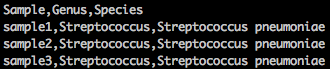
\includegraphics{img/qc_report.png}
\caption{QC report}
\end{figure}

    As we expected, these three samples are all of the same species. Let's
assume that we initially had a forth sample that we wanted to use in
this analysis. We thought that this sample was also from \textit{S.
pneumoniae}, but once we run roary with the qc option, we get the
following output:

    \begin{figure}[!h]
\centering
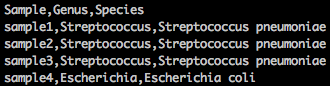
\includegraphics{img/qc_contamination.png}
\caption{QC report with contamination}
\end{figure}

    This tells us that the most prevalent species in sample 4 is in fact
\textit{Escherichia coli} so we will exclude this sample from our analysis
before we carry on.

For Sanger users Kraken is already installed and is run as part of the
automated QC pipeline. To create a symlink to the Kraken report, you can
do:

\begin{verbatim}
pf qc -t lane -i 13681_1#18 -l .
\end{verbatim}

The size of the assemblies can also provide a useful hint. If one of the
assemblies is much smaller or bigger than the others there is a chance
that this is not of the same species as the rest.

\hypertarget{coverage}{%
\subsection{Coverage}\label{coverage}}

To get decent assemblies out of your raw data, you need a genome
coverage of at least 30x. For a quick estimate of your coverage, you can
divide the number of bases in your raw data with the number of bases in
the reference genome of the species. For the samples used in this
tutorial, the coverage is listed below. The genome of \textit{S.
pneumoniae} is approximately 2,200,000 bases.

\begin{longtable}[]{@{}lll@{}}
\hline
Sample & Nr of Bases & Coverage\tabularnewline
\hline
\endhead
sample1 & 262705400 & 120x\tabularnewline
sample2 & 218026200 & 99x\tabularnewline
sample3 & 173524000 & 79x\tabularnewline
\hline
\end{longtable}

\hypertarget{fragmented-assemblies}{%
\subsection{Fragmented assemblies}\label{fragmented-assemblies}}

If the assemblies are very fragmented (thousands of contigs), the genes
may be too fragmented to be of much use.

These are just some of the most basic things that you can do to make
sure your data looks alright. There is much more that can be done but we
won't go into any further detail in this tutorial.

\hypertarget{check-your-understanding}{%
\subsection{Check your understanding}\label{check-your-understanding}}

\textbf{Q5: Why is it important to QC your data?}

\textbf{Q6: You're not getting any core genes when you run Roary. What
could be the reason?}

The answers to these questions can be found \href{answers.ipynb}{here}.

    Now you should be ready to run Roary to generate a pangenome, so head to
the next section, \href{run_roary.ipynb}{Running Roary}.\\
You can also revisit the \href{prepare_data.ipynb}{previous section} or
return to the \href{index.ipynb}{index page}.


    % Add a bibliography block to the postdoc



\newpage






    \hypertarget{running-roary}{%
\section{Running Roary}\label{running-roary}}

At this stage you should have three GFF files generated by Prokka, each
in its own directory. Provided your QC looked alright, you are now ready
to run Roary to generate the pan genome.

We are going to run Roary twice, first with the default settings, and
then using MAFFT to generate a core gene alignment. For both of these
runs we will want all the annotation files in the same directory, so
lets take a copy of them to our current directory:

\begin{terminalinput}
\begin{Verbatim}[commandchars=\\\{\}]
\llap{\color{black}\LARGE\faKeyboardO\hspace{1em}} cp annotated\PYZus{}sample*/*.gff .
\end{Verbatim}
\end{terminalinput}

    \hypertarget{run-roary-with-default-settings}{%
\subsection{Run Roary with default
settings}\label{run-roary-with-default-settings}}

Running Roary with the default settings is very straightforward. All you
need to do is to run \texttt{roary\ *.gff} and it will create a pan
genome using all GFF files in the current directory. We want to run
Roary twice with different settings, so in order to keep track of our
output files from each run we will also specify an output directory
where Roary should put the results. Give the following command a go:

\begin{terminalinput}
\begin{Verbatim}[commandchars=\\\{\}]
\llap{\color{black}\LARGE\faKeyboardO\hspace{1em}} roary \PYZhy{}f output\PYZus{}no\PYZus{}alignment *.gff
\end{Verbatim}
\end{terminalinput}

    This will run for a minute or two.

We will have a closer look at the results in the next section, so for
now let us just see that there are some output files in the directroy we
asked Roary to create:

\begin{terminalinput}
\begin{Verbatim}[commandchars=\\\{\}]
\llap{\color{black}\LARGE\faKeyboardO\hspace{1em}} ls \PYZhy{}l output\PYZus{}no\PYZus{}alignment
\end{Verbatim}
\end{terminalinput}

    \hypertarget{run-roary-with-mafft}{%
\subsection{Run Roary with MAFFT}\label{run-roary-with-mafft}}

To be able to create pretty trees and cool visualisations, we want to
genereate a multi-FASTA alignment of the core genes. To do this, we will
now run Roary again, but this time with some more options.

\begin{longtable}[]{@{}ll@{}}
\hline
Option & Description\tabularnewline
\hline
\endhead
-e & Create a multiFASTA alignment of the core genes\tabularnewline
--mafft & Use with -e to use MAFFT instead of PRANK\tabularnewline
-p & Number of threads to use\tabularnewline
\hline
\end{longtable}

By default, Roary will use PRANK when the -e option is speified. It is
accurate but slow. MAFFT is less accurate but very fast so we are going
to use this instead by specifying the --mafft option. To further speed
things up, we are going to use 8 threads (the -p option). For all usage
options, you can have a look at the
\href{https://sanger-pathogens.github.io/Roary/}{Roary website}.

\begin{terminalinput}
\begin{Verbatim}[commandchars=\\\{\}]
\llap{\color{black}\LARGE\faKeyboardO\hspace{1em}} roary \PYZhy{}f output\PYZus{}with\PYZus{}alignment \PYZhy{}e \PYZhy{}\PYZhy{}mafft \PYZhy{}p \PY{l+m}{8} *.gff
\end{Verbatim}
\end{terminalinput}

    This will take a bit longer to run than the previous command, about 5
minutes. Once finished you should have a directory called
output\_with\_alignment containing the output files, this time including
a core\_gene\_alignment.aln file. Just quickly check that this is the
case and then we will head over to the next section:
\href{results.ipynb}{Exploring the results}.

\begin{terminalinput}
\begin{Verbatim}[commandchars=\\\{\}]
\llap{\color{black}\LARGE\faKeyboardO\hspace{1em}} ls \PYZhy{}l output\PYZus{}with\PYZus{}alignment
\end{Verbatim}
\end{terminalinput}

    \hypertarget{check-your-understanding}{%
\subsection{Check your understanding}\label{check-your-understanding}}

\textbf{Q7: Why do we want to run Roary with MAFFT?}\\
a) Because it's quicker than to run Roary without the -e option\\
b) To get more accurate results\\
c) To generate a core gene alignment

\textbf{Q8: Why do we use the -p otion?}\\
a) We have to when we use MAFFT\\
b) To speed up the run\\
c) To get a pretty tree

The answers to these questions can be found \href{answers.ipynb}{here}.

You can also revisit the \href{qc.ipynb}{previous section}, or go back
to the \href{index.ipynb}{index page}.


    % Add a bibliography block to the postdoc



\newpage






    \hypertarget{exploring-the-results}{%
\section{Exploring the results}\label{exploring-the-results}}

\hypertarget{output-files}{%
\subsection{Output files}\label{output-files}}

Let's have a look at the results. We will focus on the output from the
second run as this will be the same as the first run but will also
include the core gene alignment produced by MAFFT. We will start by
looking at the most important output files and after this we will look
at how you can query your pan genome and draw a simple tree form the
core gene alignment.

\hypertarget{summary_statistics.txt}{%
\subsubsection{summary\_statistics.txt}\label{summary_statistics.txt}}

The summary\_statistics.txt file contains a summary of the number of
genes in the pan, core and accessory genomes. It provides an overview of
the genes and how frequently they occur in the input isolates. Usually,
you can expect the total number of genes in this file to be about 1,000
genes per million bases of your species reference genome. In this case,
the genomes are around 2 million bases, so we would expect a total
number of genes to be in the order of 2,000. Let's have a look and see
if this is the case.

\begin{terminalinput}
\begin{Verbatim}[commandchars=\\\{\}]
\llap{\color{black}\LARGE\faKeyboardO\hspace{1em}} cat output\PYZus{}with\PYZus{}alignment/summary\PYZus{}statistics.txt
\end{Verbatim}
\end{terminalinput}

    As you can see, we have around 2,500 genes which seems about right. If
you get a lot fewer or many more genes than expected this could be an
indication of an issue with your input data, for example contamination.

\hypertarget{gene_presence_absence}{%
\subsubsection{gene\_presence\_absence}\label{gene_presence_absence}}

The gene\_presence\_absence files lists each gene and which samples it
is present in. The .csv file can be opened in Excel.

Let's have a look at the first ten lines of the file:

\begin{terminalinput}
\begin{Verbatim}[commandchars=\\\{\}]
\llap{\color{black}\LARGE\faKeyboardO\hspace{1em}} head output\PYZus{}with\PYZus{}alignment/gene\PYZus{}presence\PYZus{}absence.csv
\end{Verbatim}
\end{terminalinput}

    The columns are tab separated and contains the following information:

\begin{enumerate}
\def\labelenumi{\arabic{enumi}.}
\tightlist
\item
  The gene name (the most frequently occurring gene name from the
  sequences in the cluster)
\item
  A non unique gene name
\item
  Functional annotation (the most frequently occurring functional
  annotation from the cluster)
\item
  Number of isolates in the cluster
\item
  Number of sequences in the cluster
\item
  Average number of sequences per isolate (normally 1)
\item
  Genome fragment
\item
  Order within fragment
\item
  Accessory fragment
\item
  Accessory order within fragment
\item
  Comments on the quality of the cluster
\item
  Minimum sequence length in nucleotides of the cluster
\item
  Maximum sequence length in nucleotides of the cluster
\item
  Average sequence length in nucleotides of the cluster
\item
  Presence and absence of genes in each sample, with the corresponding
  source Gene ID
\end{enumerate}

The .Rtab file contains a tab delimited binary matrix with the precence
and abscence of each gene in each sample. This makes it easy to load
into R using the read.table function, giving you access to a number of
useful tools. The first row is the header containing the name of each
sample, and the first column contains the gene name. In the matrix, 1
indicates the gene is present in the sample and 0 indicates it is
absent.

\hypertarget{pan_genome_reference.fa}{%
\subsubsection{pan\_genome\_reference.fa}\label{pan_genome_reference.fa}}

This fasta file contains a single nucleotide sequence from each of the
clusters in the pan genome. The name of each sequence is the source
sequence ID followed by the cluster it came from. This file can be of
use for reference guided assembly, whole genome MLST or for mapping raw
reads to it.

\hypertarget{rtab}{%
\subsubsection{.Rtab}\label{rtab}}

Roary comes packaged with a script called create\_pan\_genome\_plots.R.
It requires R and the R-package ggplot2, and can be used to generate
graphs from the .Rtab files, showing how the pan genome varies as
genomes are added.

\hypertarget{accessory_binary_genes.fa.newick}{%
\subsubsection{accessory\_binary\_genes.fa.newick}\label{accessory_binary_genes.fa.newick}}

This is a tree in newick format, created using the binary presence and
absence of accessory genes. It can for example be viewed in
\href{http://tree.bio.ed.ac.uk/software/figtree/}{FigTree}. The tree is
only a quick and dirty tree, generated to provide a rough overview of
the data. To generate a more accurate tree, we will use the core gene
alignment a bit further on.

\hypertarget{core_gene_alignment.aln}{%
\subsubsection{core\_gene\_alignment.aln}\label{core_gene_alignment.aln}}

This is the multi-FASTA alignment of core genes that we created in the
second run, using MAFFT. We will soon use this as input to build a
phylogenetic tree.

\hypertarget{clustered_proteins}{%
\subsubsection{clustered\_proteins}\label{clustered_proteins}}

In this file each line lists the sequences in a cluster. We will use
this later on in the tutorial to query the pan genome.

    For more information about the different output files, including some
that we haven't mentioned here, please feel free to have a look at the
\href{https://sanger-pathogens.github.io/Roary/}{Roary web page}.

    \hypertarget{query-the-pan-genome}{%
\subsection{Query the pan genome}\label{query-the-pan-genome}}

Roary comes with a script called query\_pan\_genome that can be used to
examine the gene differences between groups of isolates. To have a look
at the usage options for this script, you can do:

\begin{verbatim}
query_pan_genome -h
\end{verbatim}

This will show you the following usage options:

\begin{verbatim}
Usage: query_pan_genome [options] *.gff
Perform set operations on the pan genome to see the gene differences
between groups of isolates.

Options: -g STR    groups filename [clustered_proteins]
         -a STR    action (union/intersection/complement/gene_multifasta/
                     difference) [union]
         -c FLOAT  percentage of isolates a gene must be in to be core [99]
         -o STR    output filename [pan_genome_results]
         -n STR    comma separated list of gene names for use with
                     gene_multifasta action
         -i STR    comma separated list of filenames, comparison set one
         -t STR    comma separated list of filenames, comparison set two
         -v        verbose output to STDOUT
         -h        this help message

Examples:
Union of genes found in isolates
         query_pan_genome -a union *.gff

Intersection of genes found in isolates (core genes)
         query_pan_genome -a intersection *.gff

Complement of genes found in isolates (accessory genes)
         query_pan_genome -a complement *.gff

Extract the sequence of each gene listed and create multi-FASTA files
         query_pan_genome -a gene_multifasta -n gryA,mecA,abc *.gff

Gene differences between sets of isolates
         query_pan_genome -a difference --input_set_one 1.gff,2.gff --input_set_two 3.gff,4.gff,5.gff

For further info see: http://sanger-pathogens.github.io/Roary/
\end{verbatim}

    As you can see, this also shows us some examples uses. Give the first
one a go, using the clustered\_proteins file in the
output\_with\_alignment:

\begin{terminalinput}
\begin{Verbatim}[commandchars=\\\{\}]
\llap{\color{black}\LARGE\faKeyboardO\hspace{1em}} query\PYZus{}pan\PYZus{}genome \PYZhy{}a union \PY{l+s+se}{\PYZbs{}}
            \PYZhy{}g output\PYZus{}with\PYZus{}alignment/clustered\PYZus{}proteins *.gff
\end{Verbatim}
\end{terminalinput}

    This will give us a file called pan\_genome\_results that contains a
list of all genes in all samples, i.e.~the pan genome. Have a look at
the first ten lines of the newly generated file:

\begin{terminalinput}
\begin{Verbatim}[commandchars=\\\{\}]
\llap{\color{black}\LARGE\faKeyboardO\hspace{1em}} head pan\PYZus{}genome\PYZus{}results
\end{Verbatim}
\end{terminalinput}

    As you can see, the list contains the names of the clusters (this is
usually the most frequently occurring gene name from the sequences in
the cluster or, if there is no gene name, a generic unique name
group\_XXX). For each cluster, there is a tab separated list of each
sample specific gene belonging in that cluster.

In a similar way, you can use query\_pan\_genome to get a list of the
core genes:

\begin{verbatim}
query_pan_genome -a intersection \
    -g output_with_alignment/clustered_proteins *.gff
\end{verbatim}

and a list of the accessory genes:

\begin{verbatim}
query_pan_genome -a complement \
    -g output_with_alignment/clustered_proteins *.gff
\end{verbatim}

query\_pan\_genome can also be used to extract the protein sequences for
genes you are particulatly interested in. Try extracting the sequences
for three genes by specifying the -n option and a comma separated list
of the cluster names:

\begin{terminalinput}
\begin{Verbatim}[commandchars=\\\{\}]
\llap{\color{black}\LARGE\faKeyboardO\hspace{1em}} query\PYZus{}pan\PYZus{}genome \PYZhy{}a gene\PYZus{}multifasta \PY{l+s+se}{\PYZbs{}}
            \PYZhy{}g output\PYZus{}with\PYZus{}alignment/clustered\PYZus{}proteins \PY{l+s+se}{\PYZbs{}}
            \PYZhy{}n patA\PYZus{}1,mnmG,hsdS\PYZus{}2 *.gff
\end{Verbatim}
\end{terminalinput}

    You should have three new files, one for each gene you specified. Have a
look at pan\_genome\_results\_patA\_1.fa:

\begin{terminalinput}
\begin{Verbatim}[commandchars=\\\{\}]
\llap{\color{black}\LARGE\faKeyboardO\hspace{1em}} cat pan\PYZus{}genome\PYZus{}results\PYZus{}patA\PYZus{}1.fa
\end{Verbatim}
\end{terminalinput}

    This multi-FASTA file contains the three protein sequences in the
specified cluster (patA\_1).

There is yet more functionality of query\_pan\_genome, but we won't go
into that here. For further information, please feel free to visit the
\href{https://sanger-pathogens.github.io/Roary/}{Roary web page}.

    \hypertarget{draw-a-tree-form-the-core-gene-alignment}{%
\subsection{Draw a tree form the core gene
alignment}\label{draw-a-tree-form-the-core-gene-alignment}}

The tree created by Roary (accessory\_binary\_genes.fa.newick) is just a
quick tree to provide a rough insight into the data. To create a more
accurate tree you can use the core gene alignment as input to a tree
building software of your choice.
\href{https://sco.h-its.org/exelixis/web/software/raxml/index.html}{RAxML}
is very accurate, however it is also fairly slow so in this tutorial we
are going to use
\href{http://www.microbesonline.org/fasttree/}{FastTree}. You don't have
to run this step, but if you want to you need to make sure FastTree is
installed on your computer first.

To create a tree in Newick format from a nucleotide alignment using a
generalized time-reversible model (the -gtr option), do:

\begin{terminalinput}
\begin{Verbatim}[commandchars=\\\{\}]
\llap{\color{black}\LARGE\faKeyboardO\hspace{1em}} FastTree \PYZhy{}nt \PYZhy{}gtr output\PYZus{}with\PYZus{}alignment/core\PYZus{}gene\PYZus{}alignment.aln \PY{l+s+se}{\PYZbs{}}
            \PYZgt{} tree.newick
\end{Verbatim}
\end{terminalinput}

    The tree in this case will look like:

\begin{verbatim}
(sample1:0.006228253,sample2:0.002364375,sample3:0.002920483);
\end{verbatim}

We can view this in FigTree, which will look something like:

\begin{figure}[!h]
\centering

\includegraphics{img/my_tree.newick.png}
\caption{Phylogenetic tree}
\end{figure}

In the event that you did not run this step, a copy of tree.newick has
been placed in the ROARY/tree/ directory for the next section of this
tutorial.

\hypertarget{check-your-understanding}{%
\subsection{Check your understanding}\label{check-your-understanding}}

\textbf{Q9: Approximately how many genes would you expect to see in the
summary\_statistics.txt file if you are working with a species with a
genome size of 5,000,000 bases?}\\
a) 500\\
b) 5000\\
c) 50,000

\textbf{Q10: What does the accessory\_binary\_genes.fa.newick file
provide?}\\
a) A pylogenetic tree ready for publishing\\
b) Nothing, it is useless\\
c) A quick insight to the data

\textbf{Q11: For query\_pan\_genome, what option should you use to get
the accessory genome?}\\
a) union\\
b) intersection\\
c) complement

The answers to these questions can be found \href{answers.ipynb}{here}.

Now that you know a bit about the output from Roary, let's make use of
them by \href{phandango.ipynb}{visualising the results using Phandango}.

You can also revisit the \href{run_roary.ipynb}{previous page}, or go
back to the \href{index.ipynb}{index page}.


    % Add a bibliography block to the postdoc



\newpage






    \hypertarget{visualising-the-results-with-phandango}{%
\section{Visualising the results with
phandango}\label{visualising-the-results-with-phandango}}

\href{http://phandango.net/}{Phandango} is a web based tool for
visualising genomic analysis results such as phylogenetic trees and the
output of Roary and other tools. Using phandango is really easy, you
just drag your files onto the browser and drop them and Phandango will
display them for you automatically. For more in depth information please
feel free to have a look around the
\href{https://github.com/jameshadfield/phandango/wiki}{phandango wiki
page}.

In this final section of the tutorial we are going to use Phandango to
look at the pylogenetic tree we generated using FastTree, and the
gene\_presence\_absence.csv file we got from Roary. Simply dragging the
two files and droping them on the phandango front page will give you the
following view:

\begin{figure}[!h]
\centering
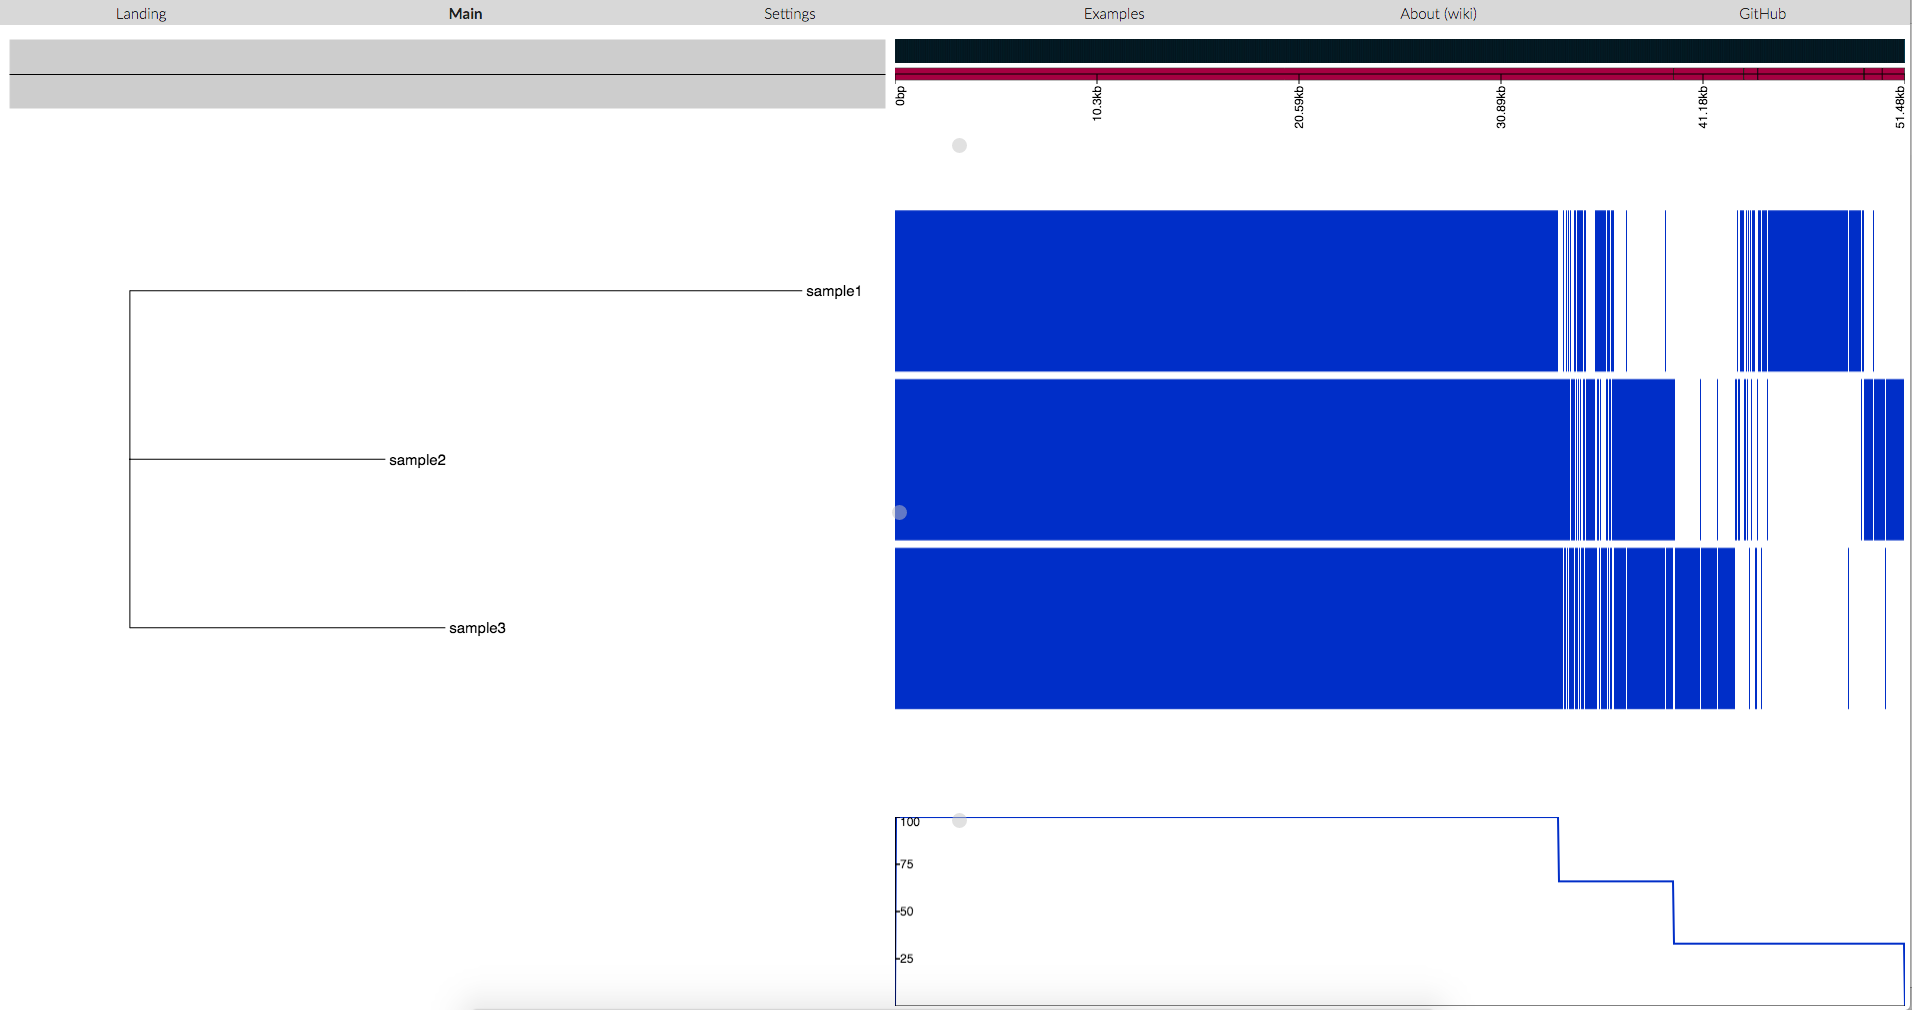
\includegraphics{img/phandango.png}
\caption{phandango}
\end{figure}

    The image shows our tree compared to a matrix with the presence and
absence of genes in the pan genome. The graph on the bottom right
provides a summary of the matrix above, indicating the percentage of
isolates carrying a gene at each position.

You can zoom in on a particular area you are interested in simply by
scrolling, and to see the annotation for a particular gene you can place
your pointer over the corresponding bar at the top of the page, like in
the figure below.

\begin{figure}[H]
\centering
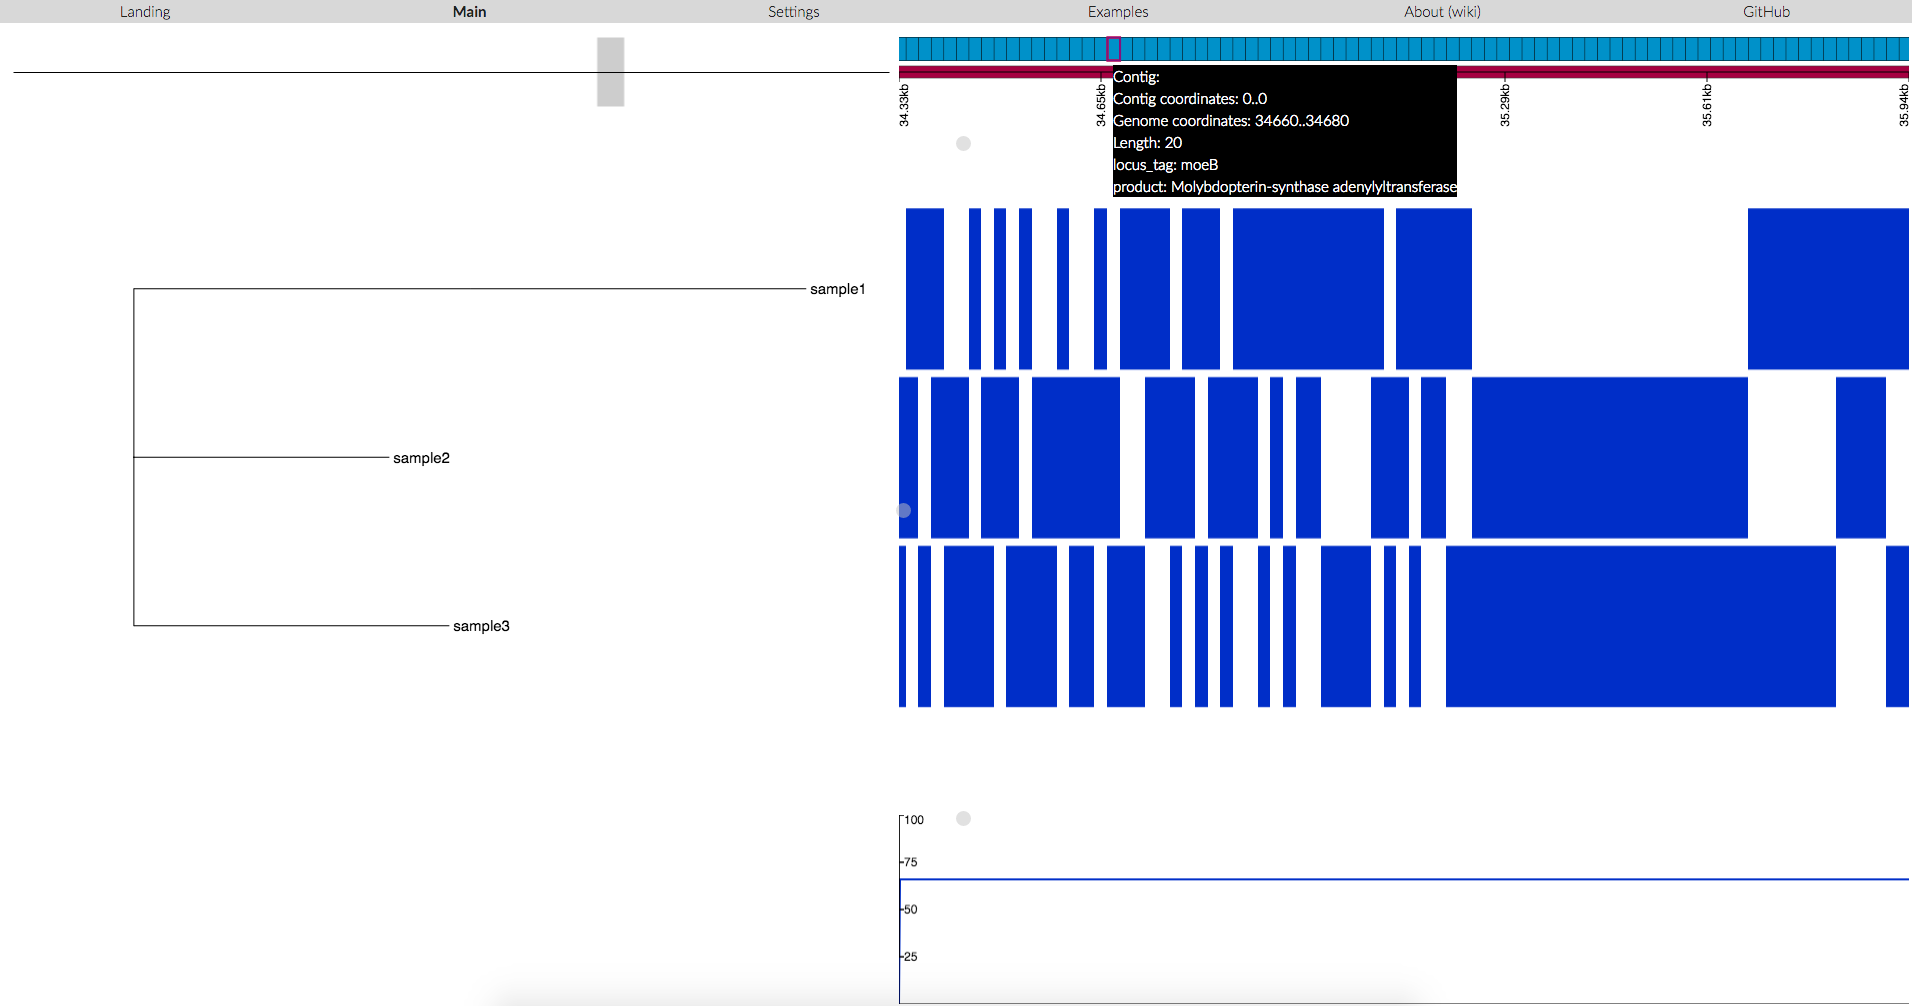
\includegraphics{img/phandango_zoom.png}
\caption{zoom}
\end{figure}

In this case we are looking at a gene called moeB. We can see that the
gene is present in sample 2 and 3, but not in sample 1, and that the
product is an Molybdopterin-synthase adenylyltransferase.

Go ahead and play around a bit in Phandango. You can alter the layout in
\textit{settings} in the navigation bar at the top of the page, or by
clicking and dragging the grey circles on the page. To download the
current view in svg format, simply press \textit{p}.

\hypertarget{check-your-understanding}{%
\subsection{Check your understanding}\label{check-your-understanding}}

\textbf{In Phandango, zoom in on the gene cluster at position 25080.}\\
\textbf{Q12: What is the name of this gene cluster?}\\
\textbf{Q13: Is this a core gene?}

The answers to these questions can be found \href{answers.ipynb}{here}.

This marks the end of this tutorial. You can either revisit the
\href{results.ipynb}{previous page} or head back to the
\href{index.ipynb}{index page}.


    % Add a bibliography block to the postdoc



\end{document}
